\documentclass[landscape, 8pt]{extarticle}

\usepackage{../../preamble}
\usepackage{symbols}

\begin{document}

\setlength{\abovedisplayskip}{3.5pt}
\setlength{\belowdisplayskip}{3.5pt}
\setlength{\abovedisplayshortskip}{3.5pt}
\setlength{\belowdisplayshortskip}{3.5pt}

\begin{multicols}{3}
\raggedcolumns


\section*{\huge General Topology Notes}
Made by Leon :) \textit{Note: Any reference numbers are to the lecture notes}

\section{Topological Spaces and Examples}

\begin{dfn}[Topological Space]{dfn:topology}{1.1}
A \textbf{topological space} is a pair $(X, \mathcal{T})$, where $X$ is a nonempty set, and $\mathcal{T}$ is a collection of subsets of $X$ which satisfies:
\begin{enumerate-a-tight}
\item $\emptyset \in \mathcal{T}$ and $X \in \mathcal{T}$
\item if $U_{\lambda}\in \mathcal{T}$ for each $\lambda\in \Lambda$ (where $\Lambda$ is some indexing set), then $\bigcup_{\lambda\in \Lambda} U_{\lambda} \in \mathcal{T}$
\item if $U_{1},\,U_{2}\in \mathcal{T}$, then $U_{1} \cap U_{2} \in \mathcal{T}$
\end{enumerate-a-tight}
The collection $\mathcal{T}$ is called the \textbf{topology} of the topological space, and the members of $\mathcal{T}$ are called the \textbf{open sets} of the topology
\end{dfn}

\begin{xmp}[Euclidean Spaces]{dfn:euclidean-spaces}{1.7}
	Let $\mathbb{R}^{n}$ denote the $n$-dimensional Euclidean vector space with elements $x = (x_{1},\,x_{2},\dots,x_{n})$ and $x_{i}\in\mathbb{R}$, and let
	\[\lvert x \rvert = \sqrt{\sum_{i = 1}^{n} x_{i}^{2}} \ge 0\]
	be the length of $x$. ($\mathbb{R}^{1} = \mathbb{R}$ is the real line). A subset $U$ of $\mathbb{R}^{n}$ is \textbf{open (for the usual topology)} iff for each $a\in U$ there exists an $r > 0$ such that
	\[\lvert x - a \rvert < r \implies x \in U.\]
	The collection of open sets thus defined is called the \textbf{usual topology} on $\mathbb{R}^{n}$. Note that open balls $B(y, \rho) = \{x\in \mathbb{R}^{n} : \lvert x - y \rvert < \rho\}$ are open sets under this definition.
\end{xmp}


\begin{xmp}[Metric Spaces]{def:metric}{1.8}
A \textbf{metric space} $(X, d)$ is a nonempty set $X$ together with a function $d : X \times X \to \mathbb{R}$ with the following properties:
\begin{enumerate-a-tight}
\item $d(x,y)\ge 0$ and $d(x,y)=0 \iff x = y$
\item $d(x,y)=d(y,x)$
\item $d(x,y)\le d(x,z)+d(z,y)$ (Triangle Inequality)
\end{enumerate-a-tight}
The function $d$ is called the \textbf{metric}.
\longrule{0.08ex}
Let $(X, d)$ be a metric space, $x$ be a point in $X$, and $r > 0$. The \textbf{open ball} with center $x$ and radius $r$ is defined by
\[B(x,r) = \{y,,\in X: d(x,y) < r\}.\]
A subset $U$ of $X$ is \textbf{open (in the metric topology given by d)} iff for each $a\in U$ there is an $r > 0$ such that $B(a,r) \subseteq U$. Just like euclidean spaces, open balls are open in this sense.
\end{xmp}


\begin{ppn}[Topology Equality]{ppn:topology-equality}{1.11}
	Let $d,\,d'$ be metrics on the same set $X$, and let $\mathcal{T},\,\mathcal{T}'$ be the corresponding metric topologies. If for real numbers $A,\, B > 0$ we have
	\[d(x, y) \le Ad'(x, y),\, d'(x, y) \le Bd(x, y) \text{ for all } x,\,y\in X,\]
	then $\mathcal{T} = \mathcal{T}'$.
\end{ppn}

% \begin{xmp}[Example of Topology Equality]{xmp:topology-equality}{1.12}
% \begin{itemize-tight}
% \item The \textbf{Euclidean metric} on $\mathbb{R}^{n}$ is defined as:
% \[d\bigl((x_{1},x_{2},\dots,x_{n}),\, (y_{1},y_{2},\dots,y_{n})\bigr) = \sqrt{\sum_{i = 1}^{n}(x_{i} - y_{i})^{2}}\]
% \item The \textbf{Box metric} on $\mathbb{R}^{n}$ is defined as:
% \[d(x, y) \le \sqrt{n} d'(x,y),\, d'(x,y) \le d(x, y)\]
% \end{itemize-tight}
% By \ref{ppn:ppn:topology-equality}, these have the same topology.
% \end{xmp}

\begin{dfn}[Subspace Topology]{dfn:subspace-topology}{1.16}
	Let $(X, \mathcal{T})$ be a topological space, and let $A \subseteq X$ be any subset. Then teh \textbf{subspace topology} on $A$ consists of all sets of the form $U \cap A$ where $U \in \mathcal{T}$.
\end{dfn}

\begin{dfn}[Closed Set]{dfn:closed-set}{1.17}
	Let $(X, \mathcal{T})$ be a topological space. A subset $A \subseteq X$ is \textbf{closed} iff its complement $X \backslash A := \{x \in X \mid x \not\in A\}$ is open in $X$. Note that a set being \textit{closed} does not mean it isn't \textit{open}. Sets that are both \textit{closed} and \textit{open} are called \textbf{clopen}.
\end{dfn}

\begin{dfn}[Properties of Topological Spaces]{dfn:topological-props}{1.20}
	For a subset $A \subseteq X$,
	\vspace{-15pt}
	\setlength{\columnseprule}{0.5pt}
	\begin{multicols}{2}
		\begin{itemize-zero}
		\item The \textbf{closure} of $A$ is
		\[\overline{A} := \bigcap_{\substack{C \subseteq X \text{ closed;}\\A \subseteq C}} C.\]
		\item The \textbf{interior} of $A$ is
		\[\Int A = A^{\circ} := \bigcap_{\substack{C \subseteq X \text{ open;} \\A \subseteq C}} C.\]
		\end{itemize-zero}
	\end{multicols}
	\vspace{-16pt}
	\begin{itemize-zero}
		\item The \textbf{boundary} (or \textbf{frontier}) of $A$ is
		\[\partial A := \overline{A} \backslash A^{\circ}.\]
		\item $A$ is \textbf{dense} in $X$ iff $\overline{A} = X$.
		\item A \textbf{limit point} of $A$ is a point $x\in X$ s.t. for every open subset $U \subseteq X$ with $x\in U$ there exists an element $a\in A \cup U$ with $a \ne x$. Let $A'$ be the set of limit points of $A$.\newline
	Note that this has nothing to do with limits of sequences.
	\end{itemize-zero}

\textrule{Proposition 1.22: Relating Toplogical Properties}
\vspace{-15pt}
\begin{itemize-zero}
	\item $\overline{A}$ is closed, and contains $A$ and is the smallest set with this property. So $A$ is closed iff $\overline{A} = A$.
	\item $A^{\circ}$ is open, and is contained in $A$, and is the largest set with this property. So $A$ is open iff $A^{\circ} = A$.
	\item The closure of the complement is the complement of the interior:
		\[\overline{X \backslash A} = X \backslash (A^{\circ}).\]
	\item The interior of the complement is the complement of the closure:
		\[(X \backslash A)^{\circ} = X \backslash \overline{A}.\]
\end{itemize-zero}

\textrule{Proposition 1.26: Union of Limit Points}
	Let $(X, \mathcal{T})$ be a topological space, and suppose $A \subseteq X$. Then
	\[\overline{A} = A \cup A'\]

\textrule{Corollary 1.27}
	A subset $A \subseteq X$ is closed iff it contains all its limit points.
\end{dfn}

\begin{thm}[Properties of open and closed sets]{thm:open-set-props}{1.19}
\vspace{-5pt}
Let $(X,\mathcal{T})$ be a topological space.
\vspace{-5pt}
\begin{enumerate-zero}
\item $\emptyset$ and $X$ are \textbf{closed}.
\item The union of \textbf{finitely many} closed sets is an closed set.
\item The intersection of \textbf{any collection} of closed sets is a closed set.
% \item The union of \textbf{any collection} of open sets is an open set.
% \item The intersection of \textbf{finitely many} open sets is an open set
\end{enumerate-zero}
\end{thm}




\begin{lma}[Limit Points and Open Balls]{lma:limit-point-balls}{1.24}
	\vspace{-5pt}
	An element $x\in X$ in a metric space $(X, d)$ is a limit point of a subset $A \subseteq X$ iff for every $\epsilon > 0$ there exists $a\in A$ with $0<d(x,a)<\epsilon$, or iff there exists a sequence $a_{1},\,a_{2},\,a_{3},\cdots$ of elements $a_{i}\in A$, with $a_{i}  \ne x$ for all $i$, s.t. $d(x_{i}, a_{i}) \to 0$ as $i \to\infty$. This interpretation does not extend to general topological spaces.
\end{lma}

\begin{thm}[Open and Closed sets in \texorpdfstring{$\mathbb{R}$}{R}]{thm:open-closed-sets-in-R}{1.30}
	\vspace{-5pt}
Consider $\mathbb{R}$ with the usual topology.
\vspace{-5pt}
\begin{enumerate-zero}
\item A nonempty set $U$ is open iff it can be written as a countable union of disjoint nonempty open intervals $I_{j}$ (shown left):
\item A set $F$ is closed iff it can be written as a countable intersection
where each $F_{j}$ is a finite union of closed intervals (shown right).
\[U = \bigcup_{j=1}^{\infty} I_{j}, \qquad F = \bigcap_{j=1}^{\infty} F_{j}.\]
\end{enumerate-zero}
\end{thm}

\begin{dfn}[Hausdorff Spaces]{dfn:hausdorff}{1.32}
	\vspace{-5pt}
	A topological space $(X, \mathcal{T})$ is \textbf{Hausdorff} if for each $x,\,y\in X$ with $x \ne y$ there exist \textbf{disjoint} open sets $U$ and $V$ such that $x\in U$ and $y\in V$.
	\longrule{0.08ex}
	Any metrisable space is Hausdorff, The trivial topology on a set with more than one element is not Hausdorff.
\end{dfn}

\begin{dfn}[Convergence of a Topological space]{dfn:convergence-topological}{1.33}
	\vspace{-5pt}
	A sequence $(x_{n})$ of members of a topological space $X$ converges to $x\in X$ if for every open set $U$ containing $x$, there exists an $N$ such that $n \ge N \implies x_{n} \in U$
\end{dfn}

\begin{ppn}[Convergence of Hausdorff Spaces]{ppn:convergence-hausdorff}{1.34}
	\vspace{-5pt}
	Suppose $(X, \mathcal{T})$ is Hausdorff. Then a sequence $(x_{n})$ can converge to at most one limit.
\end{ppn}

\begin{dfn}[Cauchy and Completeness]{dfn:cauchy-completeness}{1.36}
	\vspace{-5pt}
Let $(X, d)$ be a metric space.
\begin{enumerate-tight}
\item A \textbf{Cauchy sequence} is a sequence $(x_{n})$ with each $x_{n}\in X$ with the property that for each $\epsilon > 0$, there exists an $N$ such that $m,\,n\ge N \implies d(x_{m},\,x_{n})< \epsilon$
\item $(X, d)$ is \textbf{complete} if every Cauchy sequence converges.
\end{enumerate-tight}
\end{dfn}
\newpage

\begin{dfn}[Topology Basis]{dfn:topology-basis}{1.37}
	\vspace{-5pt}
A \textbf{basis for a topology} on a set $X$ is a collection $\mathcal{B}$ of subsets $B \subseteq X$ such that:
\begin{enumerate-tight}
\item $X = \bigcup_{B\in \mathcal{B}} B$
\item The intersection of sets $B_{1},\,B_{2}\in \mathcal{B}$ is a set $B_{1} \cap B_{2} \in \mathcal{B}$.
\end{enumerate-tight}
\vspace{-9pt}
\longrule{0.08ex}
The \textbf{topology $\mathcal{T}$ generated by a basis $\mathcal{B}$} has open sets the arbitrary unions of basis elements $B_{\lambda} \in \mathcal{B}$:
\[U = \bigcup_{\lambda\in \Lambda} B_{\lambda}\]
(Don't forget to check that this really is a topology)
\end{dfn}

\begin{xmp}[Finite Intersections of open balls]{xmp:open-balls-finite-intersections}{1.38}
	\vspace{-5pt}
	For any metric space $(X, \mathcal{T})$ the finite intersections of open balls
	\[B(x,r) = \{y \in X \mid d(x, y) < r\} \subseteq X \quad (r > 0,\, x\in X)\]
	constitute a basis for the metric topology on $X$
	\begin{multline*}
		\mathcal{B} = \{B(x_{1},r_{1}) \cap B(x_{2},r_{2}) \cap \cdots \cap B(x_{k}, r_{k}) \mid \\
		x_{1},x_{2},\dots,x_{k}\in X,\,r_{1},r_{2},\dots,r_{k}>0\}
	\end{multline*}
\end{xmp}

\section{Continuous functions and Homeomorphisms}

\begin{dfn}[Continuity]{dfn:continuity}{2.1}
	\vspace{-5pt}
	Let $(X, \mathcal{T})$, $(Y, \mathcal{U})$ be topological spaces. A function $f : X \to Y$ is \textbf{continuous} iff
	\[U \in \mathcal{U} \text{ implies } f^{-1}(U) \in \mathcal{T}.\]
	That is, \textbf{inverse} images of open sets are open. Continuous functions are often called \textbf{maps} or \textbf{mappings} of topological spaces.
\end{dfn}

\begin{ppn}[Topological and Analytic Continuity]{ppn:topological-analytic-continuity}{2.6}
	\vspace{-5pt}
	Let $(X, d)$ and $(Y, \rho)$ be metric spaces with their induced topologies $\mathcal{T}$ and $\mathcal{U}$ respectively. A function $f: X \to Y $ is continuous (topologically) iff it is continuous analytically: for every $a\in X$ and every $\epsilon > 0$ there exists $\delta > 0$ such that
	\[d(x, a) < \delta \implies \rho(f(x), f(a)) < \epsilon\]
\end{ppn}

\begin{dfn}[Homeomorphism]{dfn:homeomorphism}{2.7}
	\vspace{-5pt}
	Let $(X, \mathcal{T})$ and $(Y, \mathcal{U})$ be topological spaces. A \textbf{homeomorphism} is a bijection $f: X \to Y$ such that both $f$ and $f^{-1}$ are continuous. Two topological spaces are \textbf{homeomorphic} if there is a homeomorphism between them.
\end{dfn}


%TODO: Some stuff on topological invariants

% \begin{xmp}[Examples of homeomorphisms]{xmp:homeomorphisms}{2.10}
% \begin{enumerate-tight}
% \item Let $(X, \mathcal{T})$ be an arbitrary topological space. Then the identity map
% \[\iota : X \to X \,;\quad x \mapsto x\]
% is continuous, and indeed a homeomorphism.
% \item Suppose $(X, \mathcal{T})$, $(Y, \mathcal{U})$, and $(Z, \mathcal{W})$ are topological spaces, and that $f : X \to Y$ and $g : Y \to Z$ are continuous functions. Then their composition
% \[g \circ f : X \to Z \,; \quad x \mapsto g(f(x))\]
% is continuous.
% \item For any topological spaces $X$, $Y$, and any element $y_{0} \in Y$ the constant function
% \[f_{0} : X \to Y \,; \quad x \mapsto y_{0}\]
% is continuous.
% \end{enumerate-tight}
% \end{xmp}

% \begin{ppn}[Continuity and Closed sets]{ppn:continuity-closed}{2.14}
% \begin{itemize-zero}
% \end{itemize-zero}
% \end{ppn}

\begin{ppn}[The Punctured Sphere]{ppn:punctured-sphere}{2.18}
	\vspace{-5pt}
	Consider the $n$-dimensional sphere
	\[\mathbb{S}^{n} = \{x\in \mathbb{R}^{n+1} : \lvert x \rvert = 1\}\]
	with the metric topology inherited from $\mathbb{R}^{n+1}$. Let $x_{0} \in \mathbb{S}^{n}$. Then $\mathbb{S}^{n} \backslash \{x_{0}\}$ is homeomorphic to $\mathbb{R}^{n}$.
\end{ppn}

% TODO: whole proof

% TODO: entire section....

\section{Subspaces Revisited}

% \begin{ppn}[Hausdorff and Subspaces]{ppn:hausdorff-subspaces}{3.4}
% \end{ppn}

% \begin{ppn}[Continuity and Subspaces]{ppn:continuity-subspaces}{3.5}
% \end{ppn}
%
% \begin{crl}[Homeomorphisms and Exclusions]{crl:homeomorphisms-exclusion}{3.6}
% 	See prop A
% \end{crl}

\begin{dfn}[Disjoint Unions]{dfn:disjoint-union}{3.65}
	Let $(X, \mathcal{T})$ and $(Y, \mathcal{U})$ be topological spaces. Their \textbf{disjoint union} $X + Y$ is the set $(X \times \{0\}) \cup (Y \times \{1\})$ with the topology consisting of all sets of the form
	\[(T \times \{0\}) \cup (U \times \{1\})\text{ such that }T \in \mathcal{T},\,U \in \mathcal{U}\]
\end{dfn}

\begin{dfn}[Product Topology]{dfn:product-topology}{3.8}
	Let $(X, \mathcal{T})$, $(Y, \mathcal{U})$ be topological spaces. The \textbf{product topology} on their product $X \times Y$ consists of all sets of the form
	\[T = \bigcup_{\alpha\in A} (U_{\alpha} \times V_{\alpha})\]
	where $\mathcal{A}$ is an arbitrary indexing set, and $U_{\alpha}\in \mathcal{U}$ and $V_{\alpha}\in \mathcal{V}$.

	\textrule{Lemma 3.10}
	The product topology is indeed a topology. (lol)
\end{dfn}

\begin{lma}[Openness in Product Topologies]{lma:product-topology-open}{3.9}
	Let $(X, \mathcal{T})$ $(Y, \mathcal{U})$ be topological spaces. Then $T \subseteq X \times Y$ is open in the product topology if and only if for all $t\in T$ there exists $U \in \mathcal{U}$ and $V \in \mathcal{V}$ such that $t \in U \times V$ and $U \times V \subseteq T$.
\end{lma}

\begin{dfn}[Projection Maps]{dfn:projection-maps}{3.11.5}
	Let $(X, \mathcal{T})$ and $(Y, \mathcal{U})$ be topological spaces, and consider their product $X \times Y$ with the product topology. There are two natural maps $\Pi_{X}$ and $\Pi_{Y}$, the projections of $X \times Y$ onto $X$ and $Y$ respectively, given by
	\begin{align*}
		\Pi_{X} : X \times Y \to X, \quad (x, y) \mapsto x \\ \Pi_{Y} : X \times Y \to Y, \quad (x, y) \mapsto y.
	\end{align*}
\end{dfn}

% \begin{thm}[Continuity of Projection Maps]{thm:projection-map-continuity}{3.12}
% \end{thm}

% \begin{ppn}[Continuity of compositions]{ppn:composition-continuity}{3.13}
%
% \end{ppn}

\begin{dfn}[Weak Topology]{dfn:weak-topology}{3.14}
	Suppose that $X$ is a set. $(X_{\lambda}, \mathcal{T}_{\lambda})$ is a family of topological spaces, and that $f_{\lambda} : X \to X_{\lambda}$ are functions. The \textbf{weak topology generated by $\{f_{\lambda}\}$} is the smallest topology on $X$ making all the $f_{\lambda}$ continuous.

	Thus the product topology on $X \times Y$ is the weak topology generated by the two maps $\Pi_{X}$ and $\Pi_{Y}$
\end{dfn}

\begin{dfn}[Cartesian Product Topology]{dfn:cartesian-product}{3.15}
	If $X_{\lambda}$ is a topological space, (with $\lambda$ in some arbitrary indexing set $\Lambda$), the product topology on the cartesian product $\Pi_{\lambda\in \Lambda} X_{Ll}$ is defined to be the weak topology generated by the projections
	\[
		\Pi_{\lambda} : \prod_{\mu\in \Lambda} X_{\mu} \to X_{\lambda}
	\]
\end{dfn}

\begin{dfn}[Equivalence Relation]{dfn:equivalence-relation}{3.5.0}
An \textbf{equivalence} relation on a set $X$ is a binary operation $\sim$ on $X$ which is:
\begin{enumerate-tight}
\item \textbf{Reflexive}: $x \sim x$ for all $x\in X$.
\item \textbf{Symmetric}: if $x \sim y$ then $y \sim x$.
\item \textbf{Transitive}: if $x \sim y$ and $y \sim z$ then $x \sim z$.
\end{enumerate-tight}
The \textbf{equivalence class} of any element $x\in X$ is the set
\[[x] = \{y \in X \mid x \sim y\},\]
and the set of equivalence classes is denoted by $X / \sim$. The function which assigns to each $x\in X$ the equivalence class $[x] \in X / \sim$ is a surjection
\[p : X \to X / \sim \,; \quad x \to [x]\]
\end{dfn}


\begin{dfn}[Quotient Space]{dfn:quotient-space}{3.17}
	Given a topological space $(X, \mathcal{T})$, and an equivalence relation $\sim$ on $X$, the \textbf{quotient space} or \textbf{identification space} is the set of equivalence classes $X / \sim$ together with the topology
	\[\{ U \subseteq X / \sim : p^{-1} (U) \in \mathcal{T}\}\]
\end{dfn}

% \begin{xmp}[Circle as an Interval]{xmp:circle-interval}{3.18}
% 	The circle $S^{1}$ is homeomorphic to an identification space of the unit interval $I = [0,1]$. The topology on $I$ is defined by regarding $I$ as a subspace of $\mathbb{R}$: a subset $Y \subseteq I$ is open iff $Y = I \cup U$ for an open subset $U \subseteq \mathbb{R}$. Define an equivalence relation $\sim$ on $I$ by
% 	\[x \sim y \text{ if } x = y \text{ or if } (x, y) = (1,0) \text{ or if } (x,y) = (0,1)\]
% 	The identification space $I / \sim$ tying the two endpoints of $I$ together is homeomorphic to $S^{1}$, with a homeomorphism
% 	\[I / \sim \to S^{1}\,; \quad t \mapsto (\cos 2\pi t,\, \sin 2\pi t).\]
% 	The subset $Y = [0,1 /2) \subseteq I$ is open, since $Y = I \cup (-\infty,\,1 /2)$ with $(-\infty,\,1 /2)$ is open in $\mathbb{R}$. The image $p(Y) \subseteq I /\sim$ is not open. In fact, the open subsets $Y \subseteq I$ such that $p(Y) \subseteq I /\sim$ is open are those for which $\{0,1\} \subseteq Y$ or $\{0,1\} \cap Y = \emptyset$.
% \end{xmp}

\begin{dfn}[Generated Topological Spaces]{dfn:generator}{3.25}
	Let $X$ be a topological space, and let $Y_{0},\,Y_{1} \subseteq X$ be subspaces related by a continuous function $f: Y_{0} \to Y_{1} $. Let $\sim_{f}$ be the equivalence relation on $X$ \textbf{generated by $f$}, the intersection of all the equivalence relations on $X$ (regarded as subsets of $X \times X $) containing the pairs $(y_{0}, f(y_{0}))$ with $y_{0}\in Y_{0}$. The identification space
	\[X /\sim_{f} = X / \{ y_{1} = f(y_{0})\}\]
	is obtained by identifying each $y_{0}\in Y_{0} \subseteq X$ with $y_{1} = f(y_{0}) \in Y_{1} \subseteq X$.
\end{dfn}

% TODO: Lots of random shapes like klein bottles and tori

% \begin{ppn}[Continuity of Relations]{ppn:relation-continuity}{3.33}
% \end{ppn}

\begin{ppn}[Homeomorphisms of Relations]{ppn:relation-homeomorphisms}{3.34}
	Given a continuous function $f : X \to Y$ let $\sim$ be the equivalence relation defined on $X$ by $x \sim x'$ if $f(x) = f(x') \in Y$. The function
	\[g : X /\sim \to Y\,; [x] \to f(x)\]
	is continuous and injective, with
	\[f = g \circ p : X \prightarrow{p} X / \sim \prightarrow{g} Y.\]
	If $f$ is onto, and such that $f(U) \subseteq Y$ is open for every oopen subset $U \subseteq X$ then $g$ is a homeomorphism.
\end{ppn}
\newpage

\section{Compact Spaces}

\begin{dfn}[Open Covers and Compact Spaces]{dfn:open-cover-compact}{4.1}
\begin{enumerate-zero}
\item An \textbf{open cover} of a topological space $X$ is a collection $\{U_{\lambda} \mid \lambda\in \Lambda\}$ of open subsets $U_{\lambda}$ of $X$ such that
\[\bigcup_{\lambda\in \Lambda} U_{\lambda} = X\]

\item A topological space $X$ is \textbf{compact} if every open cover $\{U_{\lambda} \mid \lambda\in\Lambda\}$ of $X$ has a finite subcover, i.e. there exists $\lambda_{1},\dots,\lambda_{n}\in \Lambda$ such that
\[X = \bigcup_{j = 1}^{n} U_{\lambda_{j}}.\]
\end{enumerate-zero}
\textrule{Definition 4.2: Open Covers as Collections}
\vspace{-15pt}
\begin{enumerate-zero}
\item If $A \subseteq X$ is a subset of a topological space $X$, an \textbf{open cover} of $A$ is a collection $\{V_{\lambda} \mid \lambda\in\Lambda\}$ of subsets $V_{\lambda}$ which are open in $X$ such that
\[X = \bigcup_{\lambda\in\Lambda}V_{\lambda}\]
\item A subset $A$ of a toplogical space $X$ is \textbf{compact} if it is compact as a subspace of $X$.
\end{enumerate-zero}
\end{dfn}

% \begin{ppn}[Compactness and Subcoverings]{ppn:compactness-subcoverings}{4.3}
%
% \end{ppn}

% \begin{thm}[Heine-Borel Theorem]{thm:heine-borel}{4.5}
%
% \end{thm}

% \begin{ppn}[Properties of Compact Spaces]{ppn:compact-props}{4.6}
% \end{ppn}

\begin{ppn}[Boundedness of Compact Spaces]{ppn:compact-bounded}{4.7}
	A compact metric space $(X, d)$ is bounded, i.e. there exists a number $K \ge 0$ such that $d(x,y) \le K$ for all $x,\,y\in X$.
\end{ppn}

\begin{ppn}[Compactness of Products]{ppn:compact-product}{4.8}
	A product of closed bounded intervals $R = [a_{1},b_{1}] \times \cdots \times [a_{n}, b_{n}] \subseteq \mathbb{R}^{n}$ is compact in the usual topology.

	A collection of subsets of a set $X$ has the \textbf{finite intersection property} if every finite intersection of their members is nonempty.
\end{ppn}

% \begin{thm}[Compactness of Functions]{thm:compact-functions}{4.10}
%
% \end{thm}

% \begin{crl}[]{crl:compactness-invariant}{4.11}
% 	Compactness is a topological invariant. For example, $\mathbb{S}$ and $\mathbb{R}^{n}$ are not homeomorphic as the former is compact while the latter is not.
% \end{crl}

\begin{crl}[Limit Property of Compactness]{crl:compact-limit}{4.12}
	Suppose that $f : X \to \mathbb{R}^{n}$ is a continuous map and that $X$ is compact. Then there exists an $M$ such that
	\[\lvert f(x) \rvert \le M \text{ for all } x\in X.\]
	Moreover, there exists an $x\in X$ such that
	\[\lvert f(x) \rvert = \sup_{y\in X} \lvert f(y) \rvert.\]
	If $n = 1$ there are $x_{0}$ and $x_{1}\in X$ such that
	\[f(x_{0}) = \min_{x\in X} f(x) \quad \text{ and } \quad f(x_{1}) = \max_{x\in X} f(x).\]
\end{crl}

\begin{thm}[Compact,Hausdorff,Bijection, Oh My!]{thm:compact-hausdorff-bijection}{4.13}
	Suppose $X$ is compact, $Y$ is Hausdorff, and that $f : X \to Y$ is a continuous bijection. Then it is a homeomorphism.
\end{thm}


\begin{thm}[Lebesgue Numbers]{thm:lebesgue-numbers}{4.14}
	\vspace{-5pt}
	Let $X$ be a compact metric space and $\{U_{\lambda} \mid \lambda\in\Lambda\}$ an open cover of $X$. Then there exists a positive number $\delta>0$ (the \textbf{Lebesgue number} of the cover) such that for all $x\in X$, $B(x, \delta)$ lies \textit{entirely inside some single $U_{\lambda}$}.
\end{thm}

\begin{crl}[Compactness of Identification Spaces]{crl:compact-id-spaces}{4.17}
	\vspace{-5pt}
\begin{enumerate-zero}
\item An identification space $X /\sim$ of a compact space $X$ is compact.
\item If $f: X \to Y $ is a map from a compact space $X$ to a Hausdorff space $Y$ and $\sim$ is the equivalence relation on $X$ defined by $x \sim x'$ if $f(x) = f(x') \in Y$, then the continuous bijection
\[g : X / \sim \to f(X)\,;\quad [x] \mapsto f(x)\]
is a homeomorphism.
\end{enumerate-zero}
\end{crl}

% \begin{thm}[Tychonoff's Theorem - Two Products]{thm:tychonoff-simple}{4.18}
% \end{thm}

\vspace{-5pt}
\begin{lma}[Open sets in Product spaces]{lma:product-space-open-sets}{4.20}
	\vspace{-5pt}
	Let $X$ be a topological space, $Y$ a compact space, $x\in X$, $N$ an open set in $X \times Y$ such that $\{x\} \times Y \subseteq N$. Then there is an open set $W \subseteq X$ such that $x \in W$ and $W \times Y \subseteq N$.
\end{lma}

% \begin{thm}[Tychonoff's Theorem]{thm:tychonoff}{4.21}
%
% \end{thm}

\vspace{-5pt}
\begin{lma}[Collections and Intersections]{lma:collections-finite-intersections}{4.22 - 4.23}
	\vspace{-5pt}
\begin{enumerate-tight}
\item[\textbf{4.22})] Let $X$ be a set, and suppose $\mathcal{C}$ is a collection of subsets of $X$ which has the finite intersection property. Then there is a collection $\mathcal{B}$ of subsets of $X$, with $\mathcal{C} \subseteq \mathcal{B}$, such that $\mathcal{B}$ has the finite intersection property, and such that $\mathcal{B}$ is maximal with respect to this property: i.e. no collection containing $\mathcal{B}$ as a proper subcollection has the finite intersection property.
\item[\textbf{4.23})] Let $X$ be a set, and suppose that $\mathcal{B}$ is a collection of subsets of $X$ which is maximal with respect to the finite intersection property. Then $\mathcal{B}$ is closed under finite intersections, and any set which meets all members of $\mathcal{B}$ is also in $\mathcal{B}$.
\end{enumerate-tight}
\end{lma}

\vspace{-5pt}
\begin{dfn}[Compactifications]{dfn:compactifications}{4.24}
	\vspace{-5pt}
\begin{enumerate-zero}
\item A \textbf{compactification} of a topological space $X$ is a compact space $Y$ which contains a homeomorphic copy of $X$ as a subspace, i.e. such that there is a one-one map $f : X \to Y$ such that $X \to f(X)\,;\quad x \mapsto f(x)$ is a homeomorphism.
\item A compactification $Y$ is \textbf{dense} if $X$ is dense in $Y$, i.e. $\overline{X} = Y$.
\end{enumerate-zero}
\end{dfn}

% TODO: Examples

\begin{dfn}[One-point compactification]{dfn:one-point-compactification}{4.27}
	\vspace{-5pt}
The \textbf{one-point compactification} of a topological space $X$ is the set
\vspace{-5pt}
\[X^{\infty} = X \cup \{\infty\}\]
obtained by adjoining a ``point at infinity'' $\infty$, where $\infty$ is a symbol \textit{not} in $X$, with open sets of the form either
\vspace{-5pt}
\begin{enumerate-tight}
\item $U$, where $U \subseteq X$ is open, or
\item $X^{\infty} \backslash K$, where $K \subseteq X$ is compact and closed.
\end{enumerate-tight}
	\vspace{-5pt}
\textrule{Lemma 4.28}
\vspace{-15pt}
\begin{enumerate-tight}
\item The collection of open sets just defined does form a topology
\item The subspace topology on $X$ induced by this topology coincides with its original topology.
\end{enumerate-tight}
\end{dfn}

% \begin{ppn}[Compactness of OPC]{ppn:opc-compactness}{4.30}
% \end{ppn}

\begin{dfn}[Local Compactness]{dfn:local-compactness}{4.32}
	A topological space $X$ is \textbf{locally compact} if for each $x\in X$, there exists an open subset $U \subseteq X$ and a compact $C$ such that $x\in U \subseteq C$.

	\textrule{Remark 4.33}
	\vspace{-10pt}

	When $X$ is Hausdorff, it is locally compact iff for each $x\in X$ there exists an open subset $U \subseteq X$ and a compact $x \in U$ and the closure $\overline{U}$ is compact.
\end{dfn}

% \begin{ppn}[Hausdorff OPC]{ppn:hausdorff-opc}{4.34}
%
% \end{ppn}

\begin{dfn}[Normal Space]{dfn:normal-space}{4.35}
	A topological space $(X, \mathcal{T})$ is \textbf{normal} if for every pair of disjoint closed subsets $C$ and $D \subseteq X$, there are disjoint open subsets $U,\,V\subseteq X$ such that $C \subseteq U$ and $D \subseteq V$
\end{dfn}

\begin{lma}[Normal Complements]{lma:normal-complements}{4.37}
	A space $X$ is normal iff for every closed $F \subseteq X$ and open $G \subseteq X$ with $F \subseteq G$, there exist open $G'$ and closed $F'$ such that
	\[F \subseteq G' \subseteq F' \subseteq G.\]
\end{lma}

\begin{thm}[Urysohn's Lemma]{thm:urysohn}{4.38}
Suppose that $X$ is a normal topological space, and that $C,\, D$ are disjoint closed subsets of $X$. Then there is a continuous function $f : X \to \mathbb{R}$ such that
\begin{itemize-tight}
\item $f(x) = 0$ for all $x \in C$
\item $f(x) = 1$ for all $x\in D$
\item $0 \le f(x) \le 1$ for all $x\in X$
\end{itemize-tight}
\end{thm}

\begin{thm}[Tietze extension theorem]{thm:tietze-extension}{4.39}
Suppose that $X$ is a normal topological space, and that $C$ is a closed subset of $X$. Suppose that $f : C \to \mathbb{R}$ is continuous. Then there is a continuous function $\overline{f} : X \to \mathbb{R}$ such that
\begin{itemize-tight}
\item $\overline{f}(x) = f(x)$ for all $x\in C$
\item If $a \le f(x) \le b$ for all $x\in C$, then $a \le \overline{f}(x) \le b$ for all $x\in X$.
\end{itemize-tight}
\end{thm}

\begin{thm}[Stone-Weierstrass Theorem]{thm:stone-weierstrass}{4.40}
\vspace{-2pt}
	The algebra $A$ is dense in the normed space $C(X)$, i.e. $\overline{A} = C(X)$, i.e. for all $f\in C(X)$ and for all $\epsilon > 0$ there is $g\in A$ such that $\sup_{x\in X} \lvert f(x) - g(x) \rvert < \epsilon$
\end{thm}

\newpage
\section{Connected Spaces}

\begin{dfn}[Connected Spaces]{dfn:connect-spaces}{5.1}
	\vspace{-5pt}
\begin{enumerate-tight}
\item A topological space $X$ is \textbf{connected} if it \textit{cannot} be written as a union
\[X = A \cup B\]
where $A$ and $B$ are disjoint nonempty open subsets of $X$
\item A topological space $X$ is \textbf{disconnected} if it is not connected, i.e. if it \textit{can} be expressed as a union
\[X = A \cup B\]
where $A$ and $B$ are disjoint nonempty open subsets of $X$
\end{enumerate-tight}
Connectedness is a \textbf{Topological Property} (See P6).
\end{dfn}

% \begin{rem}[]{rem:connected-clopen}{5.2}
% \end{rem}

% Examples

% \begin{thm}[Connectedness of \texorpdfstring{$\mathbb{R}$}{R}]{thm:r-is-conneted}{5.4}
% \end{thm}

% \begin{thm}[Connectedness of Functions]{thm:connected-functions}{5.5}
%
% \end{thm}

\begin{rem}[Connected Homeomorphisms]{rem:connected-homeos}{5.8}
	\vspace{-5pt}
\begin{itemize-zero}
\item If $X$ is a compact connected metric space with exactly two points $x$ such that $X \backslash \{x\}$ is connected, then $X$ is homeomorphic to $[0,1]$
\item If $X$ is a compact connected space, where for every pair of distinct points $x,\, y\in X$ the complement $X \backslash \{x,y\}$ is disconnected, then $X$ is homeomorphic to the circle $\mathbb{S}_{1}$
\end{itemize-zero}
\end{rem}

% \begin{ppn}[Connected Squeeze theorem]{ppn:connected-squeeze}{5.9}
% \end{ppn}

% \begin{crl}[Connected Intervals]{crl:connected-intervals}{5.10}
% \end{crl}

\begin{ppn}[Connectedness other properties]{ppn:conneted-related-props}{5.11}
	\vspace{-5pt}
	The following statements about a nonempty subset $A \subseteq \mathbb{R}$ are equivalent:
	\begin{enumerate-tight}
		\item $A$ is connected
		\item $A$ has the interval property
		\item $A$ is an interval
	\end{enumerate-tight}
\end{ppn}

\begin{thm}[Intermediate Value Theorem]{thm:ivt}{5.12}
	\vspace{-5pt}
	Let $I$ be a closed bounded interval and suppose $f : I \to \mathbb{R}$ is continuous. Then the image $f(I)$ is a closed bounded interval
	\[f(I) = [a,b] \subseteq \mathbb{R} (a \le b).\]
\end{thm}

\begin{dfn}[Fixed Points of Maps]{dfn:fixed-point-map}{5.13}
	\vspace{-5pt}
	A \textbf{fixed point} of a map $f : X \to X$ is an $x\in X$ s.t. $f(x) = x$.
\end{dfn}

\begin{thm}[1-D Brouwer Fixed Point Theorem]{thm:1d-brouwer}{5.15}
	\vspace{-5pt}
	Every continuous map $f : [0,1] \to [0,1]$ has a fixed point, i.e. there exists $x\in[0,1]$ such that $f(x) = x$.

	General Case: Every continuous map $f : \mathbb{D}^{n} \to \mathbb{D}^{n}$ has a fixed point
\end{thm}

\begin{dfn}[Path]{dfn:path}{5.16}
	\vspace{-5pt}
	A \textbf{path} in a topological space $X$ is a continuous map $\alpha : I = [0,1] \to X$. Its \textbf{initial point} is $\alpha(0)\in X$ and its \textbf{terminal point} is $\alpha(1)\in X$.

	% TODO: put the image here?
\end{dfn}

\begin{dfn}[Path Connectedness]{dfn:path-connected}{5.18}
	A topological psace $X$ is \textbf{path-connected} if for any two points $x_{0},\,x_{1}\in X$ there exists a path $\alpha : I \to X$ from $\alpha(0) = x_{0}$ to $\alpha(1) = x_{1}$.
\end{dfn}

% \begin{thm}[Path Connectedness and Continuity]{thm:path-conn-cont}{5.18}
% \end{thm}

% \begin{crl}[Path-Connectedness Property]{crl:path-connected-prop}{5.21}
% 	see prop A
% \end{crl}

% \begin{ppn}[Path-Connectedness and ID Spaces]{ppn:path-connected-id-spaces}{5.22}
% \end{ppn}

\begin{thm}[Homeomorphisms of Real Spaces]{thm:rn-not-homeo-r}{5.24}
	If $n \ge 2$, the spaces $\mathbb{R}^{n}$ and $\mathbb{R}$ are not homeomorphic.

	Additionally, there is no bijection $f : \mathbb{R} \to \mathbb{R}^{n}$ which is continuous.
\end{thm}

% \begin{thm}[Connected means Path-Connected]{thm:connected-path-connected}{5.25}
%
% 	Note that the converse is not ture, and a connected space need not be path-connected (Example 5.2.7).
%
% 	\textrule{Theorem 5.2.8}
%
% \end{thm}

% \begin{lma}[Connected Families]{lma:connected-families}{5.30}
% \end{lma}

\begin{dfn}[Connected Components]{dfn:connected-component}{5.35}
	We define an equivalence relation $\sim$ on a topological space $x$ by $x \sim y$ iff there is a connected subset of $X$ which contains both $x$ and $y$. The resulting equivalence classes are called the \textbf{components} or \textbf{connected components} of $X$. For two homeomorphic topologial spaces there will be a bijection between the sets of their components. So spaces with differing numbers of components cannot be homemorphic. The components are the maximal connected subsets of a topological space and by Prop 5.9 are always closed in $X$. If we take $U \subseteq \mathbb{R}$ an open set, its connected component decomposition is its canonical representation as in Thm 1.30 as a countable disjoint union of open intervals.
\end{dfn}

% TODO: condense this

\begin{lma}[Path Components]{lma:path-components}{5.31.5}
Define a path (equivalence) relation
\begin{multline*}x_{0} \sim x_{1} \text{ if there exists a path } \alpha : I \to X \\ \text{ from }\alpha(0) = x_{0}\in X \text{ to } \alpha(1) = x_{1}\in X.\end{multline*}

	\begin{enumerate-tight}
		\item[\textbf{5.32})] The \textbf{constant path} at $x\in X$ is the path
		\[\alpha_{x} : I \to X \,; \quad t \mapsto x\]
		from $\alpha_{x}(0) = x\in X$ to $\alpha_{x}(1) = x\in X$
		\item[\textbf{5.33})] The \textbf{reverse} of a path $\alpha : I \to X$ is the path
		\[-\alpha : I \to X\,; \quad t\mapsto \alpha(1 - t)\]
		retracting $\alpha$ backwards, with
		% https://q.uiver.app/#q=WzAsNCxbMCwwLCItXFxhbHBoYSgwKSA9IFxcYWxwaGEoMSkiXSxbMiwwLCItXFxhbHBoYSgxKSA9IFxcYWxwaGEoMCkiXSxbMCwxLCJcXGJ1bGxldCJdLFsyLDEsIlxcYnVsbGV0Il0sWzIsMywiLVxcYWxwaGEiXSxbMCwyLCIiLDAseyJjb2xvdXIiOlswLDAsNTBdLCJzdHlsZSI6eyJoZWFkIjp7Im5hbWUiOiJub25lIn19fV0sWzEsMywiIiwyLHsiY29sb3VyIjpbMCwwLDUwXSwic3R5bGUiOnsiYm9keSI6eyJuYW1lIjoiZGFzaGVkIn0sImhlYWQiOnsibmFtZSI6Im5vbmUifX19XV0=
		\[\begin{tikzcd}[cramped,row sep=tiny]
				{-\alpha(0) = \alpha(1)} && {-\alpha(1) = \alpha(0)} \\
				\bullet && \bullet
				\arrow[color={rgb,255:red,128;green,128;blue,128}, no head, from=1-1, to=2-1]
				\arrow[color={rgb,255:red,128;green,128;blue,128}, dashed, no head, from=1-3, to=2-3]
				\arrow["{-\alpha}", from=2-1, to=2-3]
		\end{tikzcd}\]
	\item[\textbf{5.34})] The \textbf{concatenation} of paths $\alpha : I \to X,\, \beta : I \to X$ with
		\[\alpha(1) = \beta(0) \in X\]
		is the path
		\[\alpha \bullet \beta : I \to X,\;\quad t \mapsto \begin{cases}
			\alpha(2t) & \text{if } 0 \le t \le 1 /2\\
			\beta(2t - 1) & \text{if } 1 /2 \le t \le 1
		\end{cases}\]
		which starts at $\alpha(0)$, follows along $\alpha$ at twice the speed in the first half, switching at $\alpha(1) = \beta(0)$ to follow $\beta$ at twice the speed in the second half.
% https://q.uiver.app/#q=WzAsNixbMCwwLCJcXGFscGhhIFxcYnVsbGV0IFxcYmV0YSgwKSA9IFxcYWxwaGEoMCkiXSxbMiwwLCJcXGFscGhhKDEpID0gXFxiZXRhKDApIl0sWzAsMSwiXFxidWxsZXQiXSxbMiwxLCJcXGJ1bGxldCJdLFs0LDEsIlxcYnVsbGV0Il0sWzQsMCwiXFxiZXRhKDEpID0gXFxhbHBoYSBcXGJ1bGxldCBcXGJldGEoMSkiXSxbMiwzLCJcXGFscGhhIl0sWzAsMiwiIiwwLHsiY29sb3VyIjpbMCwwLDUwXSwic3R5bGUiOnsiaGVhZCI6eyJuYW1lIjoibm9uZSJ9fX1dLFsxLDMsIiIsMix7ImNvbG91ciI6WzAsMCw1MF0sInN0eWxlIjp7ImJvZHkiOnsibmFtZSI6ImRhc2hlZCJ9LCJoZWFkIjp7Im5hbWUiOiJub25lIn19fV0sWzMsNCwiXFxiZXRhIl0sWzUsNCwiIiwyLHsiY29sb3VyIjpbMCwwLDUwXSwic3R5bGUiOnsiYm9keSI6eyJuYW1lIjoiZGFzaGVkIn19fV1d
		\[\begin{tikzcd}[cramped,row sep=tiny, column sep=small]
	{\alpha \bullet \beta(0) = \alpha(0)} && {\alpha(1) = \beta(0)} && {\beta(1) = \alpha \bullet \beta(1)} \\
	\bullet && \bullet && \bullet
	\arrow[color={rgb,255:red,128;green,128;blue,128}, no head, from=1-1, to=2-1]
	\arrow[color={rgb,255:red,128;green,128;blue,128}, dashed, no head, from=1-3, to=2-3]
	\arrow[color={rgb,255:red,128;green,128;blue,128}, dashed, from=1-5, to=2-5]
	\arrow["\alpha", from=2-1, to=2-3]
	\arrow["\beta", from=2-3, to=2-5]
\end{tikzcd}\]
	\end{enumerate-tight}
\end{lma}


\begin{lma}[Connected Compomennts and Openness]{lma:connected-component-open}{5.31}
	Let $X$ be a topological space and $C$ a connected component of $X$. Then $C$ is open iff for all $x\in C$ there is an open connected $V$ such that $x\in V \subseteq C$.
\end{lma}


\begin{ppn}[Equivalence of Path Relations]{ppn:path-relation-equivalence}{5.35}
	The path relation defined on a space $X$ by $x_{0} \sim x_{1}$ if there exists a path $\alpha : I \to X$ from $\alpha(0) = x_{0}$ to $\alpha(1) = x_{0}$ is an equivalence relation.
\end{ppn}

\begin{dfn}[Path Compoments Formally]{dfn:path-components}{5.36}
	Let $X$ be a topological space.
	\begin{enumerate}
	    \item The \textbf{path compoments} of $X$ are the equivalence classes of the path equivalence relation $\sim$, i.e. the subspaces
			\begin{align*}
				[x] &= \{y\in X \mid y \sim x\}\\
					&= \{y\in X \mid \exists \alpha : I \to X \text{ from } a(0)= x \text{ to } \alpha(1)= y\}
			\end{align*}

		\item The \textbf{set of path components} (which may be infinite) is denoted by
			\[X /\sim = \pi_{0}(X)\]
		\item The function
			\[X \to \pi_{0}(X),\;\quad x \mapsto [x] = \{\text{equivalence class of }x\}\]
			is surjective.
	\end{enumerate}
\end{dfn}

% \begin{ppn}[Invariance of Path Components]{ppn:path-compoment-invariance}{5.37}
% \end{ppn}

% TODO: example 5.38

\begin{lma}[Open Condition of Path Compoments]{lma:path-compoment-open}{5.39}
	Let $X$ be a topological space and $P$ a path compoment of $X$. Then $P$ is open iff for all $x\in P$ there is an open path connected $V$ such that $x\in V \subseteq P$.
\end{lma}

\begin{lma}[Openness and Singular Components]{lma:open-singular-comp}{5.40}
	Let $C$ be a connected component of a topological space $X$. If every path component $P \subseteq C$ is open, then $C$ consists of a single path component. Note that the converse of this is not true.
\end{lma}
%
% \begin{thm}[Path Connectedness and Openness]{thm:path-connected-open}{5.41}
% \end{thm}

\newpage
\section{Relations between Top Props}
\begin{ppn}[Topological Invariants]{ppn:invariants}{A}
	A \textbf{topological property} of a topological space is one which is \textbf{invariant} under homeomorphism. Let $f : (X, \mathcal{T}) \to (Y, \mathcal{U})$ be a homeomorphism. The following properties are true:

	\begin{itemize}
		\item[\textbf{2.8})] $\mathcal{U}$ is open in $Y$ iff $f^{-1}(\mathcal{U})$ is open in $X$.
		\item $X$ is Hausdorff iff $Y$ is Hausdorff.
		\item[\textbf{3.6})] $X \backslash \{x_{0}\}$ is homeomorphic to $Y \backslash \{f(x_{0})\}$.
		\item[\textbf{4.11})] $X$ is compact, iff $Y$ is compact.
		\item[\textbf{5.6})] $X$ is connected iff $Y$ is connected.
		\item[\textbf{5.21})] $X$ is path-connected iff $Y$ is path-connected.
		\item[\textbf{5.37})] There exists a bijection between the set of path compomements $\pi_{0}(X)$ and $\pi_{0}(Y)$. However, existence of a bijection between $\pi_{0}(X)$ and $\pi_{0}(Y)$ does \textit{not} necessarily imply that $X$ and $Y$ are homeomorphic.
	\end{itemize}
\end{ppn}

\begin{ppn}[Hausdorff if...]{ppn:if-hausdorff}{B}
	\begin{itemize-tight}
		\item[\textbf{3.4})] Suppose $(X, \mathcal{T})$ is a Hausdorff topological space and suppose $A$ is a subspace. Then $A$ is Hausdorff.
		\item[\textbf{4.34})] The one-point compactification $X^{\infty}$ of a space $X$ is Hausdorff iff $X$ is Hausdorff and locally compact.
	\end{itemize-tight}
\end{ppn}

\begin{ppn}[Compact if...]{ppn:then-compact}{C}
	\begin{itemize-tight}
		\item[\textbf{4.3})] Let $X$ be a topological space and $A \subseteq X$. Then $A$ is compact iff every open cover of $A$ has a finite subcover.
		\item[\textbf{4.5})] \textbf{Heine-Borel Theorem}: A subset $F \subseteq \mathbb{R}^{n}$ is compact iff it is closed and bounded.
		\item[\textbf{4.6})] Let $X$ be a topological space and $A \subseteq X$.
			\begin{enumerate-zero}
				\item If $X$ is compact and $A$ is closed, then $A$ is compact
				\item If $X$ is Hausdorff and $A$ is compact, then $A$ is closed.
			\end{enumerate-zero}
		\item[\textbf{4.10})] Let $f : X \to Y$ be a continuous map between topological spaces. If $X$ is compact, so is $f(X)$.
		\item[\textbf{4.18})] \textbf{Tychonoff's Theorem}: Suppose $X$ and $Y$ are compact spaces. Then their product $X \times Y$ is compact. The converse is also true.
		\item[\textbf{4.21})] \textbf{Tychonoff's Theorem (General)}: Suppose that $\mathcal{A}$ is an indexing set and that for ech $\alpha\in \mathcal{A}$, $X_{\alpha}$ is a compact topological space. Then the product $\prod_{\alpha\in \mathcal{A}} X_{\alpha}$ is compact.
		\item[\textbf{4.30})] Suppose $X^{\infty} = X \cup \{\infty\}$ is the \textit{one-point compactification} of $X$. Then either $X^{\infty}$ is compact, or $X$ is dense in $X^{\infty}$
	\end{itemize-tight}
\end{ppn}

\begin{ppn}[Continuous if..]{ppn:continuity-properties}{D}
	\begin{itemize}
		\item[\textbf{2.14})] Suppose $(X, \mathcal{T})$ and $(Y, \mathcal{U})$ are topological spaces and that $f : X \to Y$. Then $f$ is continuous iff for every closed subset $F \subseteq Y$ its inverse image $f^{-1}(F)$ is closed in $X$.
		\item[\textbf{2.14})] $f$ is continuous iff the image of the closure of every subset $A \subseteq X$ is contained in the closure of the image, i.e., $\forall A \subseteq X$,
			\[f(\overline{A}) \subseteq \overline{f(A)}\]
		\item[\textbf{3.5})] Suppose $(X, \mathcal{T})$ and $(Y, \mathcal{U})$ are topological spaces and suppose $A$ is a subspace of $X$. Let $f: X \to Y $ be continuous. Then $f \rvert_{A} : A \to Y$ is continuous.
		\item[\textbf{3.12})] Let $(X, \mathcal{T})$ and $(Y, \mathcal{U})$ be topological spaces and $\mathcal{T}$ the product topology on $X \times Y$. Then the projection maps $\Pi_{X}$ and $\Pi_{Y}$ are continuous. Moreover, $\mathcal{T}$ is the smallest topology on $X \times Y$ such that the projection maps are continuous.
		\item[\textbf{3.13})] Let $X,\,Y,\,Z$ be topological spaces. Endow $X \times Y$ with the product topology. A function $f : Z \to X \times Y$ is continuous iff the functions $\Pi_{X} \circ f : Z \to X$ and $\Pi_{Y} \circ f : Z \to Y$ are both continuous.
	\end{itemize}

	\longrule{0.08ex}

	Let $X$ be a topological space with an equivalence relation $\sim$.
	\begin{enumerate-zero}
		\item The function $p: X \to X / \sim \,; \quad x \mapsto [x] $ is continuous.
		\item A continuous function $f : X \to Y$ such that $f(x) = f(x')\in Y$ for all $x,\,x\in X$ with $x \sim x'$ determines a continuous function
\[g : X / \sim \to Y\,;\quad [x] \mapsto f(x)\]
such that
\[f = g \circ p : X \prightarrow{p} X /\sim \prightarrow{g} Y\]
\end{enumerate-zero}
$f = g \circ p$ is best described by a commutative triangle:
% https://q.uiver.app/#q=WzAsMyxbMCwwLCJYIl0sWzQsMCwiWSJdLFsyLDIsIlggL1xcc2ltIl0sWzAsMiwicCJdLFsyLDEsImciXSxbMCwxLCJmIl1d
\[\begin{tikzcd}[cramped, column sep=small, row sep=scriptsize]
		X &&&& Y \\
		\\
		&& {X /\sim}
		\arrow["f", from=1-1, to=1-5]
		\arrow["p", from=1-1, to=3-3]
		\arrow["g", from=3-3, to=1-5]
	\end{tikzcd}\]
In fact, every continuous function on $X$ determines an equivalence relation.
\end{ppn}


\begin{ppn}[Connected if...]{ppn:if-connected}{E}
	\begin{itemize-tight}
		\item[\textbf{5.2})] $X$ is connected iff the only subsets of $X$ which are clopen are $\emptyset$ and $X$
		\item[\textbf{5.4})] $\mathbb{R}$ with the usual topology is connected.
		\item[\textbf{5.5})] If $f: X \to Y $ is continuous and $X$ is connected, then $f(X)$ (with the subspace topology) is connected.
		\item[\textbf{5.9})] Let $A$ be a connected subsets of a topological space $X$ and suppose $A \subseteq B \subseteq \overline{A}$. Then $B$ is connected.
		\item[\textbf{5.10})] Every nonempty interval $I \subseteq \mathbb{R}$ is connected.
		\item[\textbf{5.25})] If a topological space $X$ is path-connected, then it is also connected. Note that the converse need not be true.
		\item[\textbf{5.30})] Let $A_{\lambda} \subseteq X$, $(\lambda\in\Lambda)$ be a family of connected subsets of a topological space $X$. Suppose $\bigcup_{\lambda\in\Lambda} A_{\lambda} \ne \emptyset$. Then $\bigcup_{\lambda\in\Lambda} A_{\lambda}$ is connected.
	\end{itemize-tight}
\end{ppn}

\begin{ppn}[Path-Connected if...]{ppn:if-pathconnected}{F}
	\begin{itemize-tight}
	    \item Suppose $f : X \to Y$ is a continuous map between topological spaces and that $X$ is path-connected. Then $f(X)$ is path-connected as a subspace of $Y$.
		\item For any equivalence relation $\sim$ on a path-connected space $X$ the identification space $Y = X / \sim$ is path-connected.
		\item Any connected open subset $\Omega \subseteq \mathbb{R}^{n}$ is also path-connected.
		\item Let $X$ be a topological space. Then $X$ is path connected iff $X$ is connected \textit{and} for all $x\in X$ there is an open path connected $V$ such that $x\in V$.
	\end{itemize-tight}
\end{ppn}

\newpage
\section{Examples}

\begin{xmp}[Other Topologies and Metrics]{xmp:standard-tops-and-metrics}{}
If $(X, \mathcal{T})$ is a topological space, and $X$ admits a metric whose metric topology is precisely $\mathcal{T}$, then we say that $(X, \mathcal{T})$ is \textbf{metrisable}.
\begin{itemize-tight}
\item Euclidean spaces with their usual topologies are metrisable.
\item[\textbf{1.9)}] The \textbf{Discrete Topology} is the topology of all subsets of a set $X$. We can define the \textbf{discrete metric} of $X$ to be
\[d(x, y) = \begin{cases}
		0 & \text{if } x = y \\
		1 & \text{otherwise}
	\end{cases}.\]
\item[\textbf{1.10)}] The \textbf{Trivial} or \textbf{Indiscrete Topology} is the topology $\mathcal{T} := \{\emptyset, X\}$ for a set $X$. This is a non-metrisable topology when $X$ has more than one member.
\item[\textbf{1.14)}] Let $X = \{a,\,b,\,c\}$, where $a,\,b,\,c$ are distinct. Then
\[\mathcal{T} = \{\emptyset, X, \{a\},\,\{a,b\},\,\{a,c\}\}\]
is a topology on $X$
\item[\textbf{1.15)}] Give $\mathbb{R}$ the topolgoy whose open subsets $U \subseteq \mathbb{R}$ are precisesly the subsets with finite complement $\mathbb{R} \backslash U$, or $U = \emptyset$. Then $\mathbb{R}$ with this topology is not metrisable. This is an example of a \textbf{Zariski Topology}
\end{itemize-tight}
\end{xmp}

\begin{xmp}[The Punctured Sphere]{xmp:punctured-sphere}{B}
	\begin{figure}[H]
	    \centering
    \def\svgwidth{\columnwidth}
	\import{./figures}{punctured-sphere.pdf_tex}
	    \caption{Homeomorphism of $\mathbb{S}^{2}$ to $\mathbb{R}$}
	\end{figure}
\end{xmp}

\begin{xmp}[Topological Objects]{xmp:topological objects}{C}
	\begin{figure}[H]
	    \centering
	    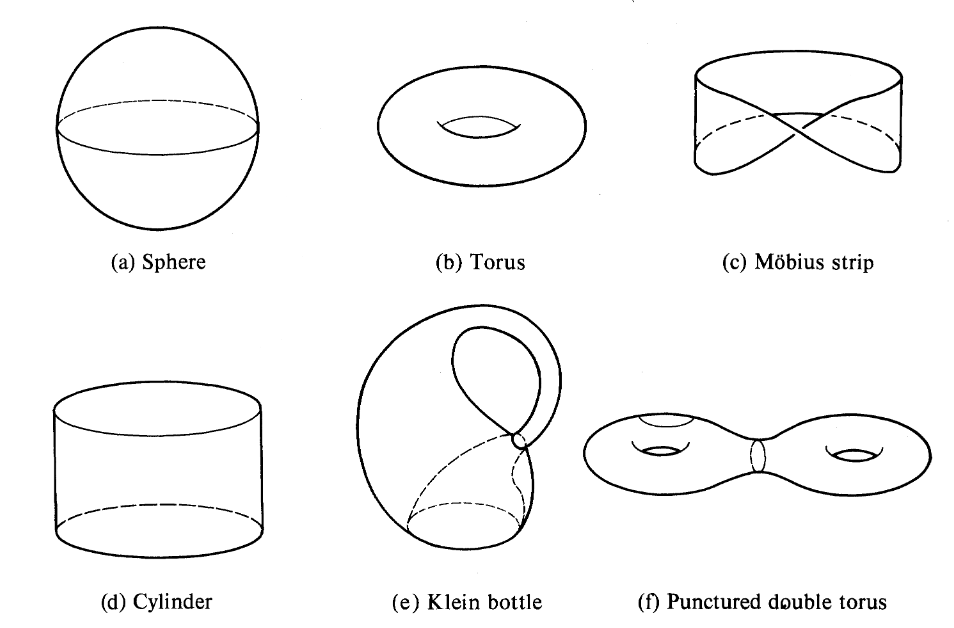
\includegraphics[width=\linewidth]{./figures/topological-objects.png}
	    \caption{Standard Topological Objects}
	\end{figure}

	\begin{multicols}{4}
	\captionsetup[figure]{name={Fig}}

	\begin{figure}[H]
		\centering
		\def\svgwidth{\columnwidth}
		\import{./figures}{mobius-construction.pdf_tex}
		\caption{M\"{o}bius Strip}
	\end{figure}

	\begin{figure}[H]
		\centering
		\def\svgwidth{\columnwidth}
		\import{./figures}{torus-construction.pdf_tex}
		\caption{Torus}
	\end{figure}

	\begin{figure}[H]
		\centering
		\def\svgwidth{\columnwidth}
		\import{./figures}{klein-construction.pdf_tex}
		\caption{Klein Bottle}
	\end{figure}
	
	\begin{figure}[H]
		\centering
		\def\svgwidth{\columnwidth}
		\import{./figures}{rp2-construction.pdf_tex}
		\caption{$\mathbb{R}\mathbb{P}^{2}$}
	\end{figure}
	    
	\end{multicols}

\end{xmp}


\end{multicols}



\end{document}
